\input{../header}
\rhead{Your name: \rule{8cm}{0.15mm}}

\begin{document}

\section{Learning target AD2, version 2}
Suppose that for some function \(p(x)\), you know the following information:
\begin{itemize}
    \item \(p(-2) = 5\),
    \item \(p'(-2) = 1.5\), 
    \item \(p''(x) < 0\) for \(x\)-values close to \(-2\). 
\end{itemize}

\begin{enumerate}[leftmargin=0pt]
    \item Explain and demonstrate how to find the linearization \(L(x)\) of \(p(x)\) at \(x =-2\). 
    \vfill
    \item Explain and demonstrate how to estimate the value of \(p(-2.03)\) using this linearization. 
    
    \vfill
    \item Is your estimate of \(p(-2.03)\) greater than or less than the actual value? How do you know?
    
    \vfill
    \item Sketch a possible graph of \(p(x)\) and its linearization \(L(x)\) nearby \(x =-2\) to illustrate your findings. Label important points in your sketch with their coordinates.
    
    \vfill
\end{enumerate}

%%%%%%%%%%%%%%%%%%%%%%%%%%%%%%%%%%%%%%%%%%%%%%%%%%%%%%%%%
\pagebreak
%%%%%%%%%%%%%%%%%%%%%%%%%%%%%%%%%%%%%%%%%%%%%%%%%%%%%%%%%

\section{Learning target AD2, version 3}

The funny thing about square roots is that most of the time, they are \textit{irrational} numbers, which means that they can't be written as fractions, and thus their decimal expansions go on forever and never repeat. For instance, \(\sqrt{67} = 8.18535277187244996995370372473392945888048681549803996306671520272366761446109794534392467163786834453471127515600621176294861011220414995972157\)

That is clearly not a particularly useful answer to the question ``what's \(\sqrt{67}\)?''
We might in particular prefer to come up with a \textit{fraction} that is a reasonably good approximation.

\begin{enumerate}[(a)]
	\item The number $\sqrt{67}$ is an output $y$-value of the function $f(x) = \sqrt{x}$. What's the corresponding input $x$-value?
	\vfill
	\item Think of an $x$-value that's close to the input value you said in part (a), but for which it is \textit{easy} to figure out the square root.

	$f(\underline{\qquad}) = \sqrt{\phantom{6464}} = \underline{\qquad}$

	\vfill
	\item Compute $f'(x)$ and plug in your easy $x$-value. Leave your answer as a fraction.

	$f'(\underline{\qquad}) = \underline{\qquad}$
	\vfill
	\item Write down the equation for the tangent line to $f(x)$ at the easy $x$-value.

	$L(x) =$
	\vfill
	\item Lastly but not leastly, plug in the hard $x$-value into the equation for the tangent line. Leave your answer as a fraction.
\end{enumerate}

%%%%%%%%%%%%%%%%%%%%%%%%%%%%%%%%%%%%%%%%%%%%%%%%%%%%%%%%%
\pagebreak
%%%%%%%%%%%%%%%%%%%%%%%%%%%%%%%%%%%%%%%%%%%%%%%%%%%%%%%%%

\section{Learning target AD2, version 4}

Part of the graph of this function $f(x)$ has been erased. 
We'll use linear approximation to recover the values.

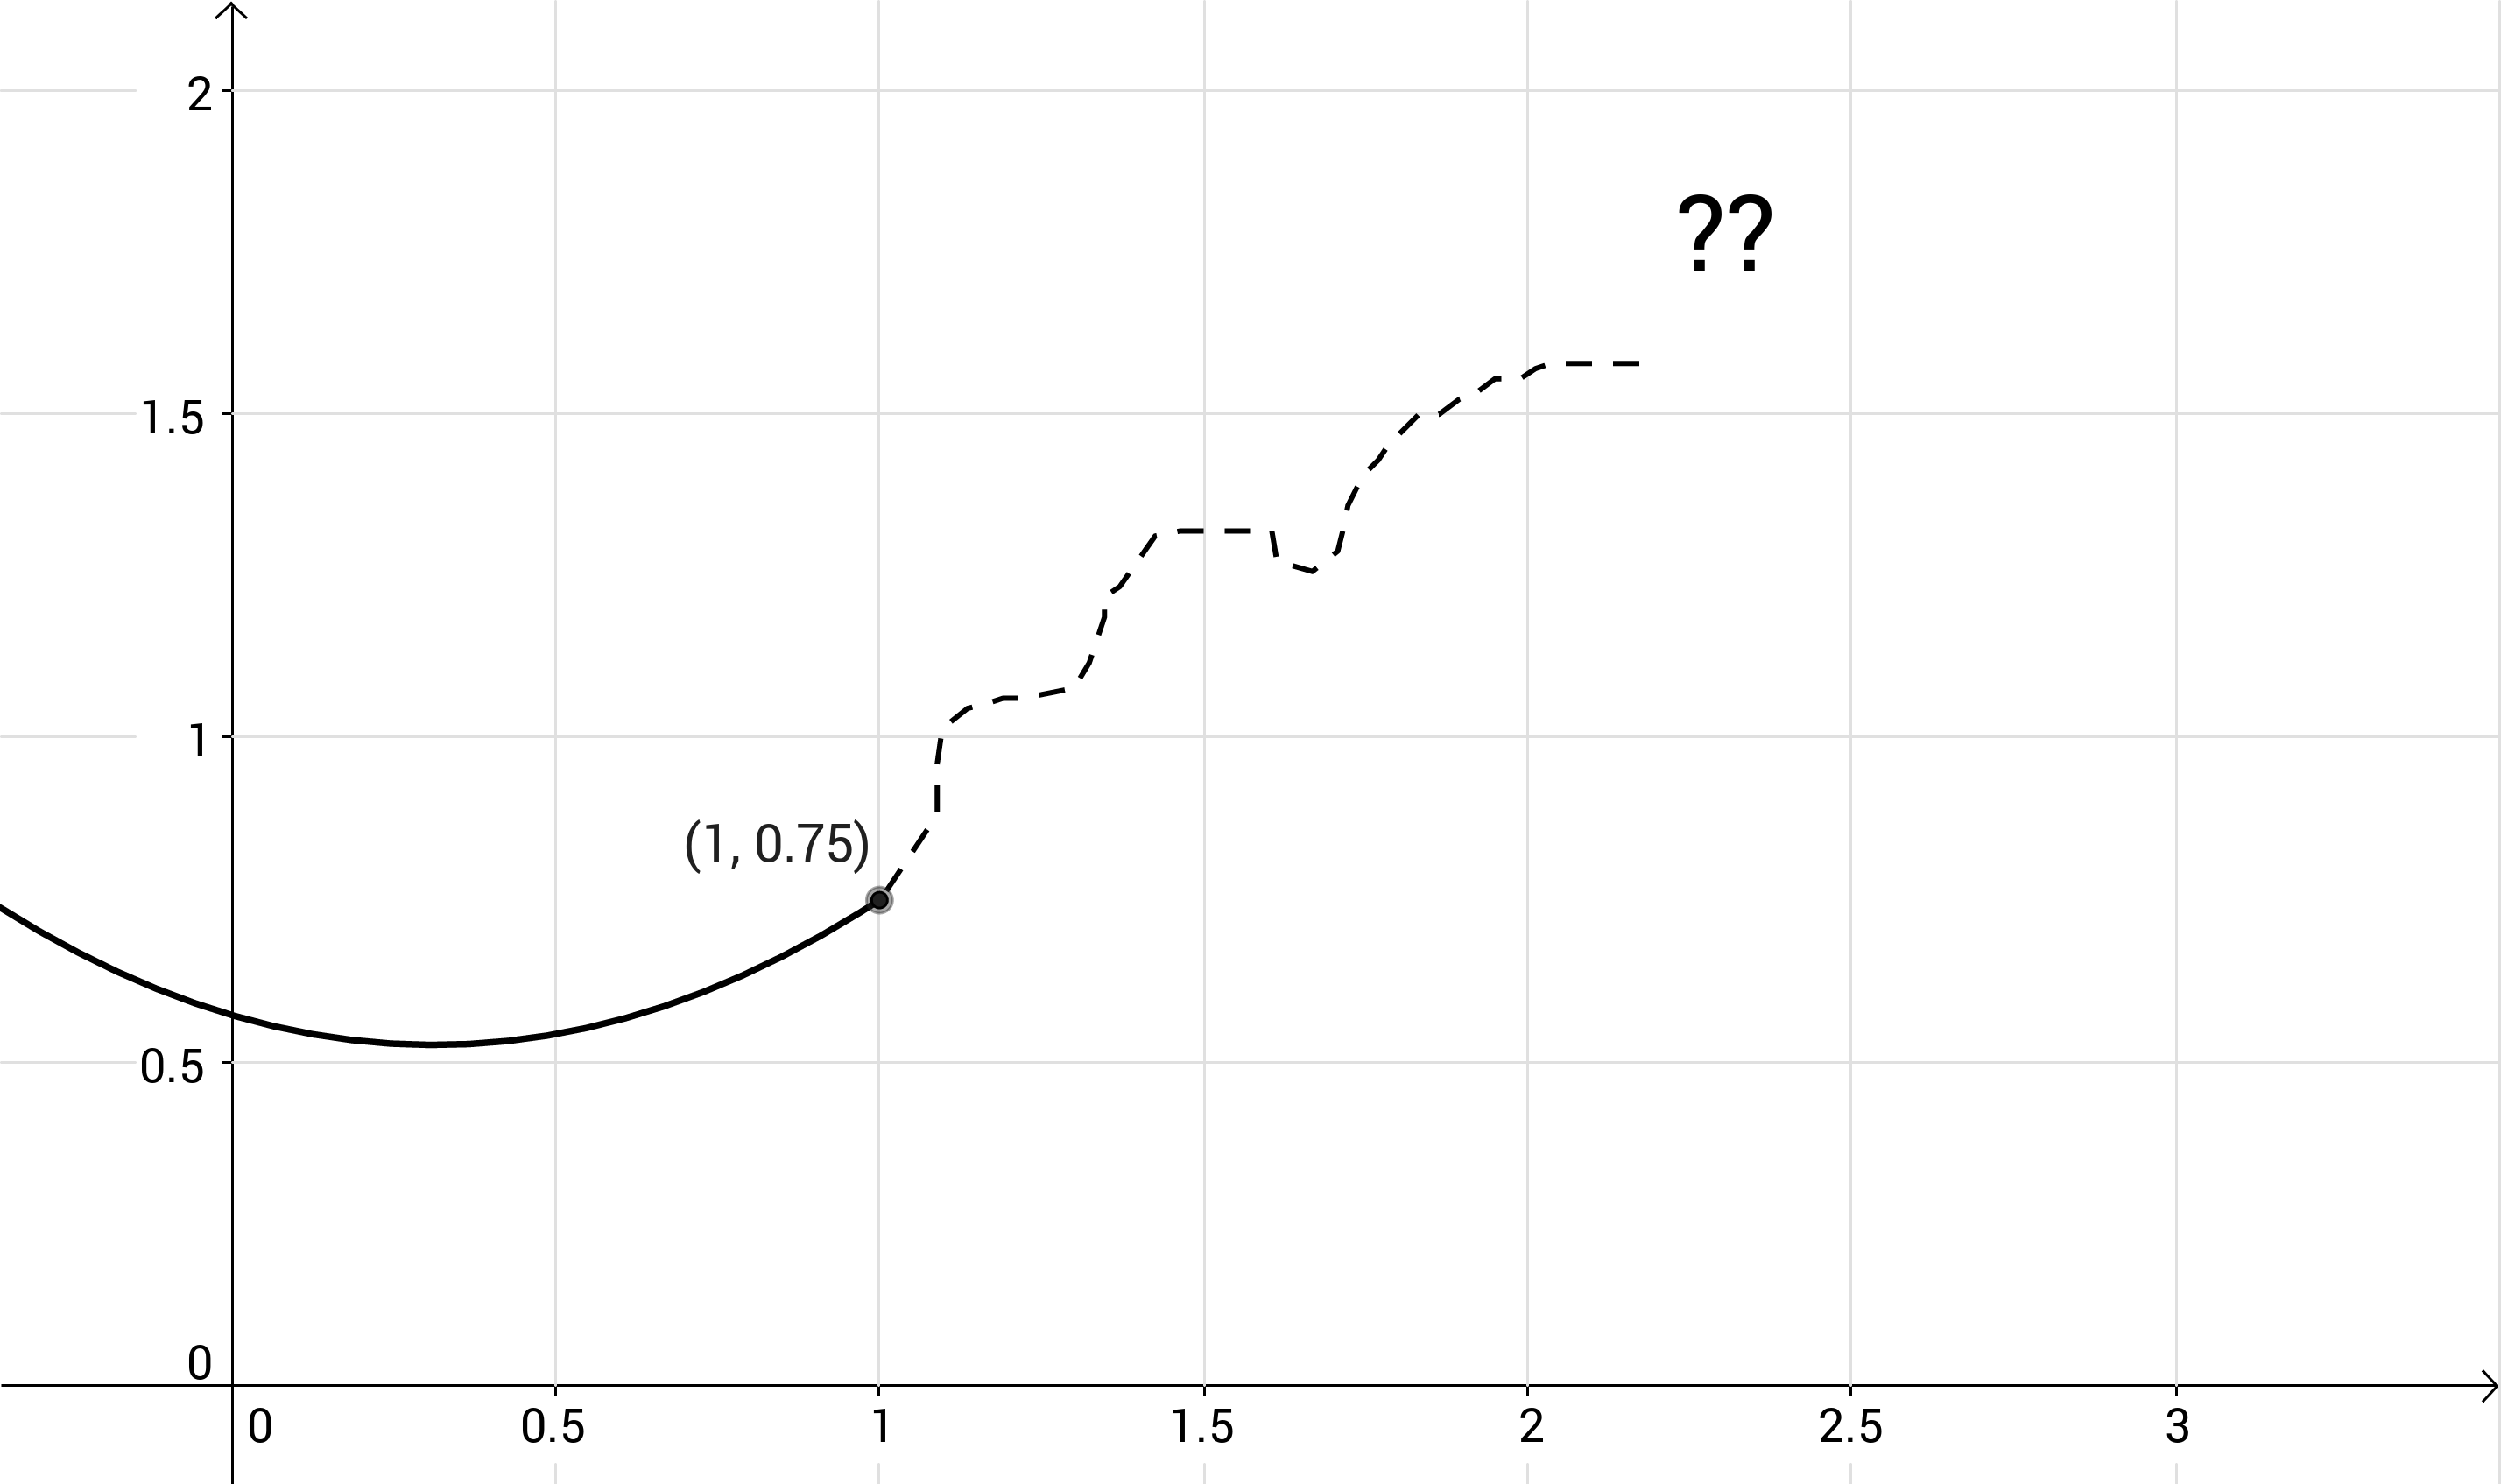
\includegraphics[width=\textwidth]{../images/linapprox.png}

\begin{enumerate}[(a)]
\item Draw the tangent line to this function at $x = 1$.
\item Suppose we know that $f'(1) = 0.65$. Use point-slope form to write down an equation for $L(x)$, the tangent line to this function at $x=1$.
\vfill
\item Use your equation for $L(x)$ to estimate $f(1.4)$.
\vfill
\item Do you think it is more likely that this is an 
overestimate or an underestimate? How come?
\vfill
\end{enumerate}

\end{document}